\chapter{Minimum Spanning Trees}

Imagine you have been handed a map of a small mountain region. There are a dozen
villages scattered across the slopes, and the regional council wants to lay
fibre-optic cable so that every village can reach every other village over the
network. Cable is expensive, and the cost of connecting two particular villages
depends on the terrain between them: some pairs are a short flat hop, others
require boring a tunnel through a ridge. You are given, for each pair of villages
that \emph{could} be connected directly, the cost of that link. Your job is to
choose a set of links so that the whole region is connected --- you can get from
any village to any other by hopping along chosen links --- while spending as
little money as possible.

That is the \emph{minimum spanning tree} problem. What makes it rewarding is that
the obvious greedy instinct --- ``keep grabbing the cheapest link you safely
can'' --- turns out to be exactly, provably right, and the reason \emph{why} it
is right is a single fact called the \emph{cut property}. Once you understand the
cut property, the two famous algorithms in this area, Kruskal's and Prim's, are
just two ways of repeatedly applying it.

\begin{focusbox}
By the end of this chapter you should be able to: (1) say precisely what a
spanning tree is and why a minimum one always exists; (2) state and \emph{feel}
the cut property, the engine behind every MST algorithm; (3) run Kruskal's
algorithm by hand, backed by a union-find structure, and Prim's algorithm by
hand, backed by a priority queue; (4) prove both correct using the cut property;
and (5) derive their running times from scratch rather than memorizing them.
\end{focusbox}

\section{What exactly are we looking for?}

Let us pin down the vocabulary before we chase any algorithm. We model the region
as a \emph{graph}. The villages are \emph{vertices}, gathered into a set $V$. The
possible direct links are \emph{edges}, gathered into a set $E$; each edge joins
two vertices. Every edge $e$ carries a number $w(e)$, its \emph{weight} --- here,
the cost of building that link. We write the graph as $G=(V,E)$ with weight
function $w$. The graph is \emph{undirected} (a cable from $u$ to $v$ is also a
cable from $v$ to $u$) and \emph{connected} (there is at least one way to get
between any two villages using available links --- otherwise no choice of edges
could ever connect everyone, and the problem has no solution).

\begin{definition}[Spanning tree]\label{ch23:def-spanning-tree}
A \emph{spanning tree} of a connected undirected graph $G=(V,E)$ is a subset
$T \subseteq E$ of the edges such that the graph $(V,T)$ is (i) \emph{connected}
--- every vertex can reach every other using only edges of $T$ --- and (ii)
\emph{acyclic} --- $T$ contains no cycle. A set of edges that is connected and
acyclic is called a \emph{tree}; ``spanning'' means it touches all of $V$.
\end{definition}

\begin{intuitionbox}
A spanning tree is the leanest possible connected skeleton of the graph. It is
\emph{connected}, so the network does its job: everyone can reach everyone.
It is \emph{acyclic}, so there is not one drop of wasted cable: a cycle would
mean two different routes between some pair of villages, and you could snip one
edge of that cycle and still keep everyone connected --- so a cycle is, by
definition, an avoidable expense.
\end{intuitionbox}

Trees have a magic counting property that we will lean on constantly: a tree on
$n$ vertices has \emph{exactly} $n-1$ edges. Fewer than $n-1$ edges cannot
connect $n$ vertices; more than $n-1$ edges on $n$ vertices must contain a cycle.
So every spanning tree of a graph with $n=|V|$ vertices uses precisely $n-1$
edges --- no algorithm can do better or worse on the \emph{count}. The only thing
left to optimize is \emph{which} $n-1$ edges.

\begin{definition}[Minimum spanning tree]\label{ch23:def-mst}
The \emph{weight} of a spanning tree $T$ is $w(T) = \sum_{e \in T} w(e)$. A
\emph{minimum spanning tree} (MST) is a spanning tree of smallest possible total
weight. (There may be several MSTs tied for the minimum; we want any one of
them.)
\end{definition}

\begin{focusbox}
Hold these three facts:
(1) A spanning tree is connected and acyclic and touches every vertex.
(2) Every spanning tree of an $n$-vertex graph has exactly $n-1$ edges.
(3) We want one whose total weight is as small as possible.
The whole chapter is about how to \emph{find} that tree without checking the
astronomically many spanning trees one by one.
\end{focusbox}

Why not just check them all? Because there are far too many. A complete graph on
$n$ vertices has $n^{n-2}$ different spanning trees (a classical result of
Cayley). For a mere $30$ villages that is already $30^{28}$, a number with $42$
digits. Brute force is hopeless. We need structure, and the structure we need is
the cut property.

\begin{aestheticbox}
MST is not a toy. It is the backbone of network design: laying water pipes,
electrical grids, road and rail networks, and --- yes --- fibre. It appears
inside clustering algorithms (delete the most expensive edges of an MST and the
tree falls into natural clusters), inside image segmentation, inside the
approximation algorithm for the travelling salesman problem you will meet much
later, and even in the wiring of computer chips. When ``connect everything as
cheaply as possible'' is the question, an MST is usually the answer.
\end{aestheticbox}

\section{A picture to anchor everything}

Let us draw a small graph and keep it on the table for the rest of the chapter.
Five villages, $a$ through $e$, with the following links and costs.

\begin{center}
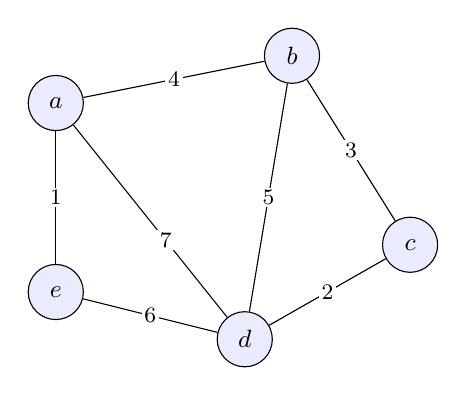
\begin{tikzpicture}[scale=1.5,
  every node/.style={font=\small},
  vert/.style={circle,draw,fill=blue!8,minimum size=7mm,inner sep=0pt},
  edgelabel/.style={fill=white,inner sep=1pt,font=\footnotesize}]
  \node[vert] (a) at (0,2)   {$a$};
  \node[vert] (b) at (2,2.4) {$b$};
  \node[vert] (c) at (3,0.8) {$c$};
  \node[vert] (d) at (1.6,0) {$d$};
  \node[vert] (e) at (0,0.4) {$e$};

  \draw (a) -- (b) node[edgelabel,midway] {$4$};
  \draw (a) -- (e) node[edgelabel,midway] {$1$};
  \draw (b) -- (c) node[edgelabel,midway] {$3$};
  \draw (b) -- (d) node[edgelabel,midway] {$5$};
  \draw (c) -- (d) node[edgelabel,midway] {$2$};
  \draw (d) -- (e) node[edgelabel,midway] {$6$};
  \draw (a) -- (d) node[edgelabel,pos=0.6] {$7$};
\end{tikzpicture}
\end{center}

Read off the edges and weights: $ae{=}1$, $cd{=}2$, $bc{=}3$, $ab{=}4$,
$bd{=}5$, $de{=}6$, $ad{=}7$. There are $5$ vertices, so every spanning tree
will use exactly $4$ edges. Spend a moment eyeballing it: the cheap edges are
$ae{=}1$, $cd{=}2$, $bc{=}3$, $ab{=}4$. Do those four edges form a spanning
tree? They connect $a$--$e$, $c$--$d$, $b$--$c$, $a$--$b$. Following the chain:
$e$--$a$--$b$--$c$--$d$. That is all five villages, no cycle, four edges. Total
cost $1+2+3+4 = 10$. We will prove later that $10$ is optimal, but you can already
sense the strategy: grab cheap edges, refuse any that would close a loop.

\section{The cut property: the heart of the matter}

Here is the single idea that makes everything work. Suppose you split the
vertices into two non-empty groups --- call this split a \emph{cut}. Some edges
have both endpoints inside the same group; those edges stay clear of the divide.
But some edges have one endpoint in each group; those edges \emph{cross} the cut.

\begin{definition}[Cut and crossing edge]\label{ch23:def-cut}
A \emph{cut} of $G=(V,E)$ is a partition of $V$ into two non-empty sets $S$ and
$V\setminus S$. An edge \emph{crosses} the cut if it has one endpoint in $S$ and
the other in $V\setminus S$. A \emph{light edge} crossing the cut is a crossing
edge of minimum weight among all edges that cross that cut.
\end{definition}

\begin{intuitionbox}
Picture a river slicing your map into a north bank ($S$) and a south bank
($V\setminus S$). Some links are entirely on one bank; the river does not touch
them. The links that span the river are the \emph{crossing} edges. Now ask: if
the final network must connect north to south, it must include \emph{at least
one} bridge across the river. Which bridge should it be? Intuitively, the
cheapest one. The cut property says that instinct is not just reasonable --- it
is guaranteed safe.
\end{intuitionbox}

Here is a concrete cut on our five-village graph. Take $S = \{a, e\}$ (shaded)
and $V \setminus S = \{b, c, d\}$. The edges \emph{inside} a side ($ae$, $bc$,
$cd$, $bd$) stay grey; the edges that \emph{cross} the cut are drawn in colour
with their weights: $ab{=}4$, $ad{=}7$, $de{=}6$. The lightest crossing edge is
$ab{=}4$, so the cut property promises $ab$ is in some MST.

\begin{center}
\begin{tikzpicture}[scale=1.5,
  every node/.style={font=\small},
  vert/.style={circle,draw,fill=blue!8,minimum size=7mm,inner sep=0pt},
  edgelabel/.style={fill=white,inner sep=1pt,font=\footnotesize}]
  \node[vert] (a) at (0,2)   {$a$};
  \node[vert] (b) at (2,2.4) {$b$};
  \node[vert] (c) at (3,0.8) {$c$};
  \node[vert] (d) at (1.6,0) {$d$};
  \node[vert] (e) at (0,0.4) {$e$};

  % shaded set S = {a,e}
  \begin{scope}[on background layer]
    \node[fill=sourceblue!15,rounded corners,fit=(a)(e),inner sep=7pt,label={[sourceblue,font=\footnotesize]above left:$S$}] {};
  \end{scope}

  % inside edges (grey)
  \draw[gray!50] (a) -- (e) node[edgelabel,midway] {$1$};
  \draw[gray!50] (b) -- (c) node[edgelabel,midway] {$3$};
  \draw[gray!50] (c) -- (d) node[edgelabel,midway] {$2$};
  \draw[gray!50] (b) -- (d) node[edgelabel,midway] {$5$};
  % crossing edges (coloured); lightest in red
  \draw[trapred,very thick] (a) -- (b) node[edgelabel,midway] {$4$};
  \draw[targetgreen!60!black,thick] (d) -- (e) node[edgelabel,midway] {$6$};
  \draw[targetgreen!60!black,thick] (a) -- (d) node[edgelabel,pos=0.6] {$7$};
\end{tikzpicture}
\end{center}

\begin{theorem}[Cut property]\label{ch23:thm-cut}
Let $G=(V,E)$ be a connected, undirected, weighted graph. Take any cut
$(S, V\setminus S)$, and let $e$ be a light edge crossing that cut (a crossing
edge of minimum weight). Then $e$ belongs to \emph{some} minimum spanning tree of
$G$.

If, in addition, all edge weights are distinct, then $e$ belongs to \emph{every}
minimum spanning tree --- the MST is unique and $e$ is forced.
\end{theorem}

Look closely at what it says. It does not require you to know anything about the
rest of the graph. Pick \emph{any} cut you like; the cheapest edge across it is
safe to commit to. That is remarkable: a purely \emph{local} decision --- look at
one cut, grab its cheapest crossing edge --- is guaranteed to be part of a
\emph{globally} optimal solution. Greedy algorithms rarely get a guarantee this
strong.

\subsection{Proof of the cut property, slowly}

We will use an \emph{exchange argument}, the workhorse technique for proving
greedy choices safe. The plan: assume someone hands you an MST that does
\emph{not} contain our light edge $e$, and show you can swap $e$ into it without
making it worse. If you can never make it worse by adding $e$, then some MST
contains $e$.

\begin{proof}
Let $e = (u,v)$ be a light edge crossing the cut $(S, V\setminus S)$, with
$u \in S$ and $v \in V\setminus S$. Let $T$ be \emph{any} minimum spanning tree.
If $e \in T$ we are already done, so assume $e \notin T$.

Now $T$ is a spanning tree, so it connects $u$ to $v$ by \emph{some} path $P$
inside $T$. (A spanning tree connects every pair of vertices, and does so by a
unique path, since trees have no cycles.) This path starts at $u$, which is in
$S$, and ends at $v$, which is in $V\setminus S$. Walking along $P$ from $u$ to
$v$, you begin on the $S$ side and finish on the other side, so \emph{somewhere}
along the way the path must step across the cut. Let $e' = (x,y)$ be an edge of
$P$ that crosses the cut, with $x \in S$ and $y \in V\setminus S$.

\begin{center}
\begin{tikzpicture}[scale=1.25,
  every node/.style={font=\small},
  vert/.style={circle,draw,minimum size=6mm,inner sep=0pt},
  Svert/.style={vert,fill=sourceblue!22},
  Tvert/.style={vert,fill=targetgreen!22}]
  % cut line
  \draw[gray!55,dashed,thick] (2.1,-0.8) -- (2.1,2.6);
  \node[gray!70] at (0.6,2.7) {$S$};
  \node[gray!70] at (3.6,2.7) {$V\setminus S$};

  \node[Svert] (u) at (0.5,1.7) {$u$};
  \node[Svert] (x) at (1.6,0.2) {$x$};
  \node[Tvert] (v) at (3.6,1.7) {$v$};
  \node[Tvert] (y) at (2.7,0.2) {$y$};

  % path P inside T
  \draw[targetgreen!60!black,thick] (u) -- (x);
  \draw[targetgreen!60!black,thick] (x) -- (y) node[midway,below,font=\footnotesize] {$e'$};
  \draw[targetgreen!60!black,thick] (y) -- (v);
  % the light edge e
  \draw[trapred,very thick] (u) -- (v) node[midway,above,font=\footnotesize] {$e$};
\end{tikzpicture}
\end{center}

Both $e$ and $e'$ cross the same cut. Since $e$ is a \emph{light} crossing edge,
$w(e) \le w(e')$.

Here is the exchange. Form a new edge set $T' = T - \{e'\} + \{e\}$: throw out
$e'$, throw in $e$. I claim $T'$ is again a spanning tree. Why? Adding $e$ to the
tree $T$ creates exactly one cycle, and that cycle consists of the new edge $e$
together with the path $P$ that already joined $u$ and $v$. The edge $e'$ lies on
$P$, hence on that cycle. Deleting any one edge of a cycle leaves the graph
connected, so removing $e'$ breaks the cycle without disconnecting anything.
After the swap we still have $|V|-1$ edges, still connected, hence still a
spanning tree.

What is its weight? We removed $e'$ and added $e$, so
$$ w(T') = w(T) - w(e') + w(e) \le w(T),$$
because $w(e) \le w(e')$. But $T$ was a \emph{minimum} spanning tree, so its
weight cannot be beaten: $w(T') \ge w(T)$. The only way to have both
$w(T') \le w(T)$ and $w(T') \ge w(T)$ is $w(T') = w(T)$. Therefore $T'$ is also a
minimum spanning tree --- and it contains $e$. So \emph{some} MST contains $e$,
which is the first claim.

For the second claim, suppose all weights are distinct. Then unless $e' = e$ we
have strict inequality $w(e) < w(e')$, which would give $w(T') < w(T)$,
contradicting that $T$ is minimum. So in fact $e' = e$, meaning $e$ was in $T$
all along. Since $T$ was an arbitrary MST, \emph{every} MST contains $e$.
\end{proof}

\begin{focusbox}
The exchange argument is worth more than the theorem. The pattern --- ``assume an
optimal solution lacks my greedy choice; find a cycle/path that lets me swap my
choice in for free; conclude an optimal solution \emph{can} contain my choice''
--- recurs throughout greedy algorithm design. Learn the move, not just the
result.
\end{focusbox}

\begin{trapbox}
The cut property does \textbf{not} say ``the globally cheapest edge of the whole
graph is in every MST.'' It says ``the cheapest edge \emph{across a given cut} is
safe.'' These coincide for the very cheapest edge (it is light across the cut
separating one of its endpoints from everything else), but for a general edge you
must name the cut. Beginners often try to argue ``this edge is the second
cheapest, so it must be in the MST'' --- false in general. Always exhibit a cut.
\end{trapbox}

\section{The generic MST algorithm}

The cut property hands us a strategy so general that it is barely an algorithm
yet --- more like a recipe with a blank to fill in. We grow a set of edges $A$
that we have committed to. We maintain one invariant: \emph{$A$ is always a
subset of some MST}. At each step we find an edge that is ``safe'' to add ---
meaning $A \cup \{e\}$ is still a subset of some MST --- and add it. When $A$ has
$|V|-1$ edges, it is a spanning tree, and since it is a subset of some MST and has
the right size, it \emph{is} that MST.

\begin{algorithm}[H]
\caption{\textsc{Generic-MST}$(G, w)$}
\KwIn{A connected weighted undirected graph $G=(V,E)$ with weights $w$.}
\KwOut{A minimum spanning tree, returned as an edge set $A$.}
$A \gets \emptyset$\;
\While{$A$ does not yet span all of $V$ \emph{(}fewer than $|V|-1$ edges\emph{)}}{
  find an edge $(u,v)$ that is \emph{safe} for $A$\;
  $A \gets A \cup \{(u,v)\}$\tcp*{commit to it}
}
\Return $A$\;
\end{algorithm}

How do we find a safe edge? The cut property gives a sufficient condition.

\begin{formalbox}
Call an edge $e$ \emph{safe} for $A$ if $A \cup \{e\}$ is a subset of some MST.
\textbf{Sufficient condition (from the cut property).} Suppose $A$ is a subset of
some MST. Choose any cut $(S, V\setminus S)$ that \emph{no edge of $A$ crosses}.
Then a light edge across that cut is safe for $A$.
\end{formalbox}

The condition ``no edge of $A$ crosses the cut'' is what guarantees the new edge
can be added to the partial solution without conflict: $A$ lives entirely within
the two sides, and we are adding the first, cheapest bridge between them. The
proof is the cut property applied to the MST that contains $A$ --- the light edge
joins $A$ rather than disturbing it.

\begin{focusbox}
Every MST algorithm in this chapter is just \textsc{Generic-MST} with a specific
rule for choosing the cut (and therefore the safe edge):
\begin{itemize}
\item \textbf{Prim} fixes one growing blob $S$ and always cuts ``blob vs.\ the
  rest,'' adding the cheapest edge leaving the blob.
\item \textbf{Kruskal} keeps a forest of blobs and adds the globally cheapest
  edge that joins two \emph{different} blobs --- which is a light edge for the cut
  separating one of those blobs from everything else.
\end{itemize}
Same engine, two steering wheels.
\end{focusbox}

\section{Kruskal's algorithm}

Kruskal's algorithm is the embodiment of the village engineer's instinct: sort
all the candidate links from cheapest to most expensive, then walk down the list
and build each one \emph{unless} it would create a redundant loop.

\subsection{The idea}

\begin{intuitionbox}
Start with $n$ villages and no cable at all --- $n$ separate islands. Sort the
links by cost. Consider them cheapest first. For each link, ask: do its two
endpoints already sit on the same island (already connected by cable laid so
far)? If yes, skip it --- building it would only close a wasteful loop. If no,
build it; this fuses two islands into one. Stop when a single island remains.
\end{intuitionbox}

Why is each accepted edge safe? Suppose we are about to accept edge $(u,v)$
because $u$ and $v$ are on different islands. Let $S$ be the island containing
$u$. No edge of $A$ crosses the cut $(S, V\setminus S)$ --- because $S$ is a
\emph{whole} connected island, every edge already built either stays inside $S$
or stays outside it. And $(u,v)$ is the cheapest edge crossing that cut that we
have seen, because we are processing edges in increasing weight order and this is
the first one we have encountered that joins $S$ to the outside. So $(u,v)$ is a
light edge for a cut that $A$ does not cross: safe, by the cut property.

\subsection{The mechanism: union-find}

The one operation we keep performing is ``are $u$ and $v$ on the same island,
and if not, fuse their islands.'' This is precisely what a \emph{disjoint-set}
(union-find) data structure is built for. You met it in the chapter on disjoint
sets; here is the contract we need.

\begin{itemize}
\item \textsc{Make-Set}$(x)$: create a one-element island $\{x\}$.
\item \textsc{Find-Set}$(x)$: return a canonical name (the ``representative'') of
  the island containing $x$. Two elements are on the same island iff their
  \textsc{Find-Set} answers are equal.
\item \textsc{Union}$(x,y)$: fuse the islands of $x$ and $y$ into one.
\end{itemize}

With \emph{union by rank} and \emph{path compression}, a sequence of $m$ of these
operations on $n$ elements costs $O(m\,\alpha(n))$, where $\alpha$ is the
inverse-Ackermann function --- so slow-growing it is at most $4$ for any input
size that fits in this universe. For our purposes you may treat each operation as
``essentially constant time.''

\subsection{The algorithm}

\begin{algorithm}[H]
\caption{\textsc{MST-Kruskal}$(G, w)$}
\KwIn{Connected weighted undirected graph $G=(V,E)$.}
\KwOut{An MST as an edge set $A$.}
$A \gets \emptyset$\;
\For{each vertex $v \in V$}{\textsc{Make-Set}$(v)$\tcp*{each village its own island}}
sort the edges of $E$ into nondecreasing order by weight $w$\;
\For{each edge $(u,v) \in E$, taken in that sorted order}{
  \If{\textsc{Find-Set}$(u) \ne$ \textsc{Find-Set}$(v)$}{
    $A \gets A \cup \{(u,v)\}$\tcp*{endpoints on different islands: safe}
    \textsc{Union}$(u,v)$\tcp*{fuse the islands}
  }
}
\Return $A$\;
\end{algorithm}

\subsection{A full trace on our graph}

Sort the edges of the five-village graph by weight:
$$ae{=}1,\quad cd{=}2,\quad bc{=}3,\quad ab{=}4,\quad bd{=}5,\quad de{=}6,\quad ad{=}7.$$
Start with five islands: $\{a\},\{b\},\{c\},\{d\},\{e\}$.

\begin{center}
\renewcommand{\arraystretch}{1.25}
\begin{tabular}{c c c l}
\toprule
edge & weight & same island? & action / islands after \\
\midrule
$ae$ & $1$ & no  & \textbf{accept}; islands $\{a,e\},\{b\},\{c\},\{d\}$ \\
$cd$ & $2$ & no  & \textbf{accept}; islands $\{a,e\},\{b\},\{c,d\}$ \\
$bc$ & $3$ & no  & \textbf{accept}; islands $\{a,e\},\{b,c,d\}$ \\
$ab$ & $4$ & no  & \textbf{accept}; islands $\{a,b,c,d,e\}$ \\
$bd$ & $5$ & yes & skip (would close cycle $b$--$c$--$d$--$b$) \\
$de$ & $6$ & yes & skip \\
$ad$ & $7$ & yes & skip \\
\bottomrule
\end{tabular}
\end{center}

We accepted $\{ae, cd, bc, ab\}$, four edges, total weight $1+2+3+4 = 10$. Once
the fourth edge merged everything into one island, every later edge had both
endpoints in that single island and was skipped. The result matches the tree we
eyeballed earlier.

\begin{center}
\begin{tikzpicture}[scale=1.5,
  every node/.style={font=\small},
  vert/.style={circle,draw,fill=blue!8,minimum size=7mm,inner sep=0pt},
  edgelabel/.style={fill=white,inner sep=1pt,font=\footnotesize}]
  \node[vert] (a) at (0,2)   {$a$};
  \node[vert] (b) at (2,2.4) {$b$};
  \node[vert] (c) at (3,0.8) {$c$};
  \node[vert] (d) at (1.6,0) {$d$};
  \node[vert] (e) at (0,0.4) {$e$};

  \draw[trapred,very thick] (a) -- (b) node[edgelabel,midway] {$4$};
  \draw[trapred,very thick] (a) -- (e) node[edgelabel,midway] {$1$};
  \draw[trapred,very thick] (b) -- (c) node[edgelabel,midway] {$3$};
  \draw[trapred,very thick] (c) -- (d) node[edgelabel,midway] {$2$};
  \draw[gray!45,dashed] (b) -- (d) node[edgelabel,midway] {$5$};
  \draw[gray!45,dashed] (d) -- (e) node[edgelabel,midway] {$6$};
  \draw[gray!45,dashed] (a) -- (d) node[edgelabel,pos=0.6] {$7$};
\end{tikzpicture}
\end{center}

\begin{labbox}
Trace Kruskal yourself on this graph. Vertices $\{1,2,3,4\}$; edges with weights
$12{=}1$, $13{=}4$, $14{=}3$, $23{=}2$, $34{=}5$. Sort the edges, walk the list,
and record the islands after each decision. You should accept three edges of
total weight $1+2+3 = 6$. Which edges? Confirm that each edge you skip would have
closed a cycle.
\end{labbox}

\subsection{Why Kruskal is correct}

\begin{theorem}\label{ch23:thm-kruskal}
\textsc{MST-Kruskal} returns a minimum spanning tree.
\end{theorem}

\begin{proof}
We show the loop invariant: \emph{at every point, $A$ is a subset of some MST}.
Initially $A = \emptyset$, which is a subset of any MST, so the invariant holds.

Suppose it holds and we are about to accept an edge $(u,v)$ because
\textsc{Find-Set}$(u) \ne$ \textsc{Find-Set}$(v)$. Let $S$ be the set of vertices
currently in the island (the union-find tree) of $u$. Two things are true. First,
no edge of $A$ crosses the cut $(S, V\setminus S)$: every edge already in $A$
joined two vertices that ended up in the \emph{same} island, so it lies wholly
inside one side. Second, $(u,v)$ is a light edge across this cut. To see this,
notice that no crossing edge of $(S, V\setminus S)$ can have been examined before
$(u,v)$. Indeed, take any edge $(x,y)$ that crosses the cut now, with $x \in S$
and $y \notin S$. The island $S$ only grew over time, so at any earlier moment
$x$ sat in some sub-island of $S$ while $y$ sat outside it; the two endpoints
were therefore in \emph{different} islands, and had we examined $(x,y)$ back then
we would have \emph{accepted} it, fusing $y$'s side into $S$ --- contradicting
that $y$ is still outside $S$. So every crossing edge is examined no earlier than
$(u,v)$. Because we scan edges in nondecreasing weight order, $(u,v)$ is no
heavier than any crossing edge, i.e.\ it is a minimum-weight crossing edge. By
the cut property,
$(u,v)$ is safe: $A \cup \{(u,v)\}$ is still a subset of some MST. The invariant
is preserved.

Edges we \emph{skip} (same island) do not change $A$, so they cannot break the
invariant. When the loop ends, $A$ is acyclic (we never added an edge inside an
island) and connected (the graph is connected, so processing all its edges must
have fused every vertex into one island; an unfused vertex would witness an edge
that crosses between islands and was wrongly skipped). Hence $A$ is a spanning
tree, and being a subset of some MST with the full $|V|-1$ edges, it \emph{is}
that MST.
\end{proof}

\subsection{Running time of Kruskal}

Let $n = |V|$ and $m = |E|$. Walk through the costs:

\begin{itemize}
\item $n$ calls to \textsc{Make-Set}: $O(n)$.
\item Sorting the $m$ edges: $O(m \log m)$. Since $m \le n^2$, $\log m \le 2\log n$,
  so this is $O(m \log n)$.
\item The main loop runs $m$ times, each doing two \textsc{Find-Set}s and at most
  one \textsc{Union}. That is $O(m)$ union-find operations, costing
  $O(m\,\alpha(n))$ in total.
\end{itemize}

\begin{complexitybox}
\textbf{Kruskal's algorithm.} Sorting dominates.
$$T(n,m) = O(m \log m) + O(m\,\alpha(n)) = O(m \log n).$$
Because $\alpha(n)$ grows slower than every $\log$, the union-find work is lost in
the noise; the bottleneck is putting the edges in sorted order. If the edges
arrive \emph{already} sorted, or can be sorted in linear time (small integer
weights), Kruskal runs in $O(m\,\alpha(n))$, essentially linear.
\end{complexitybox}

\begin{historybox}
Joseph Kruskal published this algorithm in 1956, in a short paper that was partly
about justifying a different, then-popular method. The union-find machinery that
makes it fast came later. In CLRS this material is Chapter~21 (``Minimum Spanning
Trees''), with the disjoint-set structures in Chapter~19. If you want the cut
property stated as CLRS states it, look for their Theorem~21.1.
\end{historybox}

\section{Prim's algorithm}

Kruskal grows many little trees at once and merges them. Prim takes the opposite
tack: grow \emph{one} tree, outward from a single seed, always reaching for the
cheapest edge that extends it.

\subsection{The idea}

\begin{intuitionbox}
Plant a flag on any one village; call it the start of your network. You now have a
blob $S = \{\text{start}\}$ and everyone else outside. Repeat: among all links
with exactly one endpoint inside the blob, pick the cheapest, and build it. That
link pulls one new village into the blob. Keep going until the blob swallows every
village. The links you built form the tree.
\end{intuitionbox}

This is \textsc{Generic-MST} with the cut fixed as ``the blob $S$ versus the rest''
at every step. The cheapest edge leaving the blob is a light edge across that cut,
and no edge of our growing tree crosses the cut (the tree lives entirely inside
$S$). So every edge Prim adds is safe.

\subsection{The mechanism: a priority queue}

The repeated question is now ``which outside village is cheapest to attach to the
blob, and by which edge?'' For each vertex $v$ still outside, keep a number
$key[v]$ = the weight of the cheapest edge connecting $v$ to a vertex already
inside, and $\pi[v]$ = the inside vertex at the other end of that edge. We want to
repeatedly extract the outside vertex of smallest $key$, then, when a vertex joins
the blob, update its outside neighbours in case it offers them a cheaper hookup.
``Repeatedly extract the smallest, and decrease keys'' is exactly the job of a
\emph{min-priority queue}.

\begin{algorithm}[H]
\caption{\textsc{MST-Prim}$(G, w, r)$}
\KwIn{Connected weighted undirected graph $G=(V,E)$; a start vertex $r$.}
\KwOut{For each $v$, its parent $\pi[v]$; the tree edges are $\{(v,\pi[v])\}$.}
\For{each vertex $u \in V$}{$key[u] \gets \infty$; \quad $\pi[u] \gets \textsc{Nil}$}
$key[r] \gets 0$\;
$Q \gets V$\tcp*{min-priority queue keyed by $key[\cdot]$}
\While{$Q \ne \emptyset$}{
  $u \gets$ \textsc{Extract-Min}$(Q)$\tcp*{cheapest vertex to attach now}
  \For{each neighbour $v$ of $u$}{
    \If{$v \in Q$ \textbf{and} $w(u,v) < key[v]$}{
      $\pi[v] \gets u$\;
      $key[v] \gets w(u,v)$\tcp*{Decrease-Key}
    }
  }
}
\end{algorithm}

A subtlety worth a sentence: ``$v \in Q$'' means $v$ is still outside the blob.
Once a vertex is extracted it is inside the blob forever, and its key is frozen ---
that frozen key is the weight of the edge that pulled it in.

\subsection{A full trace on our graph}

Start at $r = a$. Keys begin at $key[a]=0$, all others $\infty$. We will write the
key vector as $(a,b,c,d,e)$ and underline the vertex we extract.

\begin{center}
\renewcommand{\arraystretch}{1.3}
\begin{tabular}{c l l l}
\toprule
step & extract $u$ & edge added & keys after relaxing $u$ \\
\midrule
1 & \underline{$a$} ($0$) & --- (root) &
  $b{=}4\,(\pi a),\ d{=}7\,(\pi a),\ e{=}1\,(\pi a)$ \\
2 & \underline{$e$} ($1$) & $a\!-\!e$ &
  $d$: $de{=}6 < 7 \Rightarrow d{=}6\,(\pi e)$ \\
3 & \underline{$b$} ($4$) & $a\!-\!b$ &
  $c{=}3\,(\pi b)$; $d$: $bd{=}5 < 6 \Rightarrow d{=}5\,(\pi b)$ \\
4 & \underline{$c$} ($3$) & $b\!-\!c$ &
  $d$: $cd{=}2 < 5 \Rightarrow d{=}2\,(\pi c)$ \\
5 & \underline{$d$} ($2$) & $c\!-\!d$ & queue empty \\
\bottomrule
\end{tabular}
\end{center}

Let us narrate the interesting steps. After extracting $a$, its neighbours get
keys: $b{=}4$, $d{=}7$, $e{=}1$, each pointing back at $a$. The smallest key now
belongs to $e$, so we extract $e$ and add the edge $a\!-\!e$ (weight $1$). From
$e$ the only outside neighbour is $d$ via $de{=}6$, which beats $d$'s current
$7$, so $key[d]$ drops to $6$ with $\pi[d]=e$. Next smallest outside is $b$ at
$4$; extract it, add $a\!-\!b$. Relaxing $b$: neighbour $c$ gets $key{=}3$
($\pi c = b$), and $d$ improves from $6$ to $5$ via $bd$. Next we extract $c$ at
$3$, add $b\!-\!c$; relaxing $c$ drops $d$ from $5$ to $2$ via $cd$. Finally
extract $d$ at $2$, adding $c\!-\!d$.

Edges added: $a\!-\!e\,(1)$, $a\!-\!b\,(4)$, $b\!-\!c\,(3)$, $c\!-\!d\,(2)$.
Total $1+4+3+2 = 10$. Same tree, same cost as Kruskal --- as it must be, since
the MST here is unique.

The figure below shows the same run as a \emph{growing blob}. The shaded region
is $S$, the set of villages already pulled in; the small number on each tree edge
is its weight, and the number in a circle marks the step at which that vertex was
extracted. Watch $S$ swallow one vertex per step, always along the cheapest exit.

\begin{center}
\begin{tikzpicture}[scale=1.5,
  every node/.style={font=\small},
  vert/.style={circle,draw,fill=blue!8,minimum size=7mm,inner sep=0pt},
  edgelabel/.style={fill=white,inner sep=1pt,font=\footnotesize},
  order/.style={font=\scriptsize\bfseries,sourceblue,inner sep=1pt}]
  \node[vert] (a) at (0,2)   {$a$};
  \node[vert] (b) at (2,2.4) {$b$};
  \node[vert] (c) at (3,0.8) {$c$};
  \node[vert] (d) at (1.6,0) {$d$};
  \node[vert] (e) at (0,0.4) {$e$};

  % shaded blob over all five (final S)
  \begin{scope}[on background layer]
    \node[fill=sourceblue!12,rounded corners,fit=(a)(b)(c)(d)(e),inner sep=8pt] {};
  \end{scope}

  \draw[trapred,very thick] (a) -- (b) node[edgelabel,midway] {$4$};
  \draw[trapred,very thick] (a) -- (e) node[edgelabel,midway] {$1$};
  \draw[trapred,very thick] (b) -- (c) node[edgelabel,midway] {$3$};
  \draw[trapred,very thick] (c) -- (d) node[edgelabel,midway] {$2$};
  \draw[gray!45,dashed] (b) -- (d) node[edgelabel,midway] {$5$};
  \draw[gray!45,dashed] (d) -- (e) node[edgelabel,midway] {$6$};
  \draw[gray!45,dashed] (a) -- (d) node[edgelabel,pos=0.6] {$7$};

  % extraction order labels
  \node[order] at (-0.35,2.35) {1};
  \node[order] at (-0.35,0.75) {2};
  \node[order] at (2.35,2.75) {3};
  \node[order] at (3.4,1.15) {4};
  \node[order] at (1.95,0.35) {5};
\end{tikzpicture}
\end{center}

\begin{trapbox}
Notice that $key[d]$ was lowered \emph{four} times --- from $\infty$ to $7$, then
$6$, then $5$, then $2$ --- before $d$ was finally extracted. That is the whole point of
\textsc{Decrease-Key}: a vertex's cheapest connection keeps improving as the blob
grows and gets closer to it. The value frozen at extraction time ($2$, via $cd$)
is the one that lands in the tree. A common bug is to ``lock in'' a vertex's
parent the first time you see it; you must keep relaxing until it is extracted.
\end{trapbox}

\subsection{Why Prim is correct}

\begin{theorem}\label{ch23:thm-prim}
\textsc{MST-Prim} computes a minimum spanning tree.
\end{theorem}

\begin{proof}
Let $A = \{(v,\pi[v]) : v \ne r,\ v \notin Q\}$ be the set of tree edges
collected so far --- the edges of vertices already extracted. We claim $A$ is
always a subset of some MST. Initially $A = \emptyset$: fine.

Consider the moment we extract a vertex $u$ (other than $r$) and thereby add edge
$(u, \pi[u])$ to $A$. Let $S$ be the set of vertices already inside the blob just
before this extraction (the previously extracted vertices). No edge of $A$ crosses
the cut $(S, V\setminus S)$, since every edge of $A$ joins two already-extracted
vertices, both in $S$. We must check that $(u,\pi[u])$ is a light edge across this
cut. Each outside vertex $v$ has $key[v]$ equal to the weight of the cheapest edge
from $v$ into $S$ (that is the invariant the relaxation loop maintains), and
\textsc{Extract-Min} chose $u$ as the outside vertex with smallest such key. So
$w(u,\pi[u]) = key[u]$ is the minimum over all outside vertices of their cheapest
edge into $S$ --- precisely the minimum-weight edge crossing the cut. By the cut
property, $(u,\pi[u])$ is safe, and the invariant survives. When $Q$ empties,
every vertex is in the blob, $A$ has $|V|-1$ edges, and being a subset of an MST
of the right size, it \emph{is} an MST.
\end{proof}

\subsection{Running time of Prim}

The cost depends entirely on the priority queue. The algorithm performs:

\begin{itemize}
\item $|V|$ \textsc{Extract-Min} operations (one per vertex), and
\item at most $|E|$ \textsc{Decrease-Key} operations (each edge $(u,v)$ can
  trigger at most one key decrease for $v$ when $u$ is extracted; summed over the
  graph, the relaxation loop runs $\sum_v \deg(v) = 2|E|$ times).
\end{itemize}

So the running time is
$$|V|\cdot t_{\text{extract}} + |E|\cdot t_{\text{decrease}},$$
and we just plug in the queue's costs.

\begin{center}
\renewcommand{\arraystretch}{1.35}
\begin{tabular}{l c c l}
\toprule
priority queue & \textsc{Extract-Min} & \textsc{Decrease-Key} & total time \\
\midrule
unsorted array      & $O(n)$        & $O(1)$           & $O(n^2 + m) = O(n^2)$ \\
binary heap         & $O(\log n)$   & $O(\log n)$      & $O((n+m)\log n) = O(m\log n)$ \\
Fibonacci heap      & $O(\log n)$\,* & $O(1)$\,*        & $O(m + n\log n)$ \\
\bottomrule
\end{tabular}
\end{center}

(The Fibonacci-heap bounds are \emph{amortized}, marked $*$.) With a binary heap
Prim matches Kruskal at $O(m \log n)$. With a Fibonacci heap Prim reaches
$O(m + n\log n)$, which is asymptotically better on \emph{dense} graphs where
$m$ is close to $n^2$. And for a truly dense graph the humble unsorted array,
at $O(n^2)$, can beat the heap, since $O(n^2) = O(m)$ when $m = \Theta(n^2)$ and
there is no $\log$ factor to pay.

\begin{complexitybox}
\textbf{Prim's algorithm.}
\begin{itemize}
\item Binary heap: $O(m \log n)$ --- the standard, all-purpose choice.
\item Fibonacci heap: $O(m + n \log n)$ --- best for dense graphs, in theory.
\item Array: $O(n^2)$ --- simplest, and best when $m \approx n^2$.
\end{itemize}
\textbf{Kruskal's algorithm.} $O(m \log n)$, dominated by sorting the edges.
On sparse graphs the two are tied; on dense graphs the right Prim variant wins.
\end{complexitybox}

\begin{historybox}
The algorithm is named for Robert Prim (1957), though Vojt\v{e}ch Jarn\'ik
described it back in 1930 and Edsger Dijkstra rediscovered it in 1959 --- so you
will sometimes see it called the Jarn\'ik--Prim or Prim--Dijkstra algorithm.
Notice how closely \textsc{MST-Prim} resembles Dijkstra's shortest-path
algorithm, which you will meet in the next chapter: both grow a blob by repeatedly
extracting the minimum-key frontier vertex. The difference is one line --- Prim's
key is ``weight of the single connecting edge,'' Dijkstra's key is ``total
distance from the source.'' CLRS Chapter~21 covers both Kruskal and Prim.
\end{historybox}

\section{Kruskal vs.\ Prim: which, and why}

\begin{intuitionbox}
\textbf{Kruskal} thinks globally about edges: sort everything, take the cheapest
that does not loop. It grows a \emph{forest} of many trees that gradually merge.
It is the natural choice when the edges are few (sparse graph) or already sorted.

\textbf{Prim} thinks locally about one tree: keep extending a single blob along
its cheapest exit. It grows \emph{one} tree from a seed. It shines on dense
graphs, especially with a good priority queue, because it never has to sort all
the edges at once --- it only ever looks at edges on the current frontier.
\end{intuitionbox}

Both rest on the same foundation --- the cut property --- and both return a
correct MST. They differ only in \emph{which cut} they apply the property to at
each step. One theorem thus gives rise to a family of algorithms, each making the
abstract ``find a safe edge'' step concrete in its own way.

\begin{walkbox}
Here is something to chew on during a walk. The cut property guarantees the
cheapest edge across any cut is in \emph{some} MST. Is there a matching ``cycle
property''? Try to convince yourself that the \emph{most expensive} edge on any
cycle can be safely \emph{excluded} from some MST. (Hint: mirror the exchange
argument --- if an MST contained that heaviest cycle edge, swap it out for the
edge that closes the cycle.) If both properties hold, you have two ways to think
about every MST: include light cut edges, exclude heavy cycle edges. They are two
faces of the same coin.
\end{walkbox}

\section{A few subtleties}

\begin{remark}[Ties and uniqueness]
If all edge weights are distinct, the MST is unique (the cut property, second
half, forces every light edge). When weights tie, several MSTs may exist; both
algorithms still return a valid one, but \emph{which} one can depend on tie-break
order. Nothing about correctness changes --- all of them have the same minimum
total weight.
\end{remark}

\begin{remark}[Disconnected graphs]
We assumed $G$ is connected. If it is not, no spanning tree exists. Both
algorithms then produce a \emph{minimum spanning forest}: Kruskal naturally
yields one tree per connected component; Prim from a single seed only reaches the
seed's component, so you would restart it on an unreached vertex.
\end{remark}

\begin{remark}[Negative weights are fine]
Unlike some shortest-path algorithms, MST algorithms do not care if weights are
negative. The cut property never assumed positivity --- ``cheapest crossing
edge'' makes perfect sense whether costs are $+5$ or $-5$. You could add a huge
constant to every weight; the same tree stays minimal, since every spanning tree
has the same number of edges, so all their weights shift by the same amount.
\end{remark}

\section*{Looking back}

We started with a single, concrete worry --- connect the villages as cheaply as
possible --- and uncovered a structure so clean it almost feels unfair. One
theorem, the cut property, says local greed is globally safe. One generic
procedure repeatedly grabs a safe edge. Two famous algorithms, Kruskal and Prim,
are just two ways of choosing the cut to look at. And the analysis bottoms out in
two data structures you already know: union-find for Kruskal, a priority queue for
Prim. When you reach CLRS Chapter~21, you will find these same ideas stated more
tersely --- but you will recognize every move, because you built them here from
the ground up.

\section{Exercises}

\begin{exercise}\label{ch23:ex-byhand}
Run both Kruskal and Prim (start Prim at vertex $1$) on this graph and confirm
they produce the same tree and total weight. Vertices $\{1,2,3,4,5\}$; edges
$12{=}2$, $13{=}3$, $24{=}5$, $34{=}4$, $35{=}6$, $45{=}1$, $25{=}7$. Show your
island merges (Kruskal) and your key vector at each extraction (Prim).
\end{exercise}

\begin{exercise}\label{ch23:ex-count}
A connected graph has $100$ vertices. Exactly how many edges does \emph{any} of
its spanning trees contain? Explain in one sentence why the count cannot depend
on which spanning tree you pick.
\end{exercise}

\begin{exercise}\label{ch23:ex-cheapest-edge}
Prove that the single cheapest edge of a connected graph (assume a unique
minimum-weight edge) belongs to every MST. (Hint: find a cut for which it is the
light edge.)
\end{exercise}

\begin{exercise}\label{ch23:ex-cycle-property}
\textbf{Cycle property.} Let $C$ be any cycle in $G$, and let $e$ be a
strictly-heaviest edge on $C$ (assume it is the unique heaviest edge of $C$).
Prove that $e$ belongs to \emph{no} MST. Use an exchange argument that mirrors the
proof of the cut property.
\end{exercise}

\begin{exercise}\label{ch23:ex-maximum}
Suppose you wanted a \emph{maximum}-weight spanning tree instead (the most
expensive connected acyclic skeleton). Describe the smallest change to Kruskal's
algorithm that solves it, and argue briefly why your change is correct.
\end{exercise}

\begin{exercise}\label{ch23:ex-unique}
Prove that if every edge weight in $G$ is distinct, then $G$ has exactly one
minimum spanning tree. (You may use the second half of the cut property.)
\end{exercise}

\begin{exercise}\label{ch23:ex-prim-array}
For a complete graph on $n$ vertices ($m = \binom{n}{2}$), compare the running
time of Prim with a binary heap, $O(m\log n)$, against Prim with an unsorted
array, $O(n^2)$. Which is asymptotically faster here, and by what factor? When
would you still prefer the heap?
\end{exercise}

\begin{exercise}\label{ch23:ex-bottleneck}
\textbf{Challenge (bottleneck spanning tree).} The \emph{bottleneck} of a
spanning tree is the weight of its single heaviest edge. Prove that every minimum
spanning tree is also a \emph{minimum-bottleneck} spanning tree --- that is, no
spanning tree has a smaller heaviest edge. (Is the converse true? Find a small
counterexample showing a minimum-bottleneck tree need not be an MST.)
\end{exercise}

\begin{exercise}\label{ch23:ex-add-edge}
You have already computed an MST $T$ of a graph $G$. Now a single new edge
$(u,v)$ with weight $w$ is added to $G$. Describe an $O(n)$-time method to update
the MST, and justify it using the cycle property from
Exercise~\ref{ch23:ex-cycle-property}. (Hint: adding $(u,v)$ to $T$ creates one
cycle.)
\end{exercise}

\begin{exercise}\label{ch23:ex-unionfind-why}
In Kruskal's algorithm, why is the union-find structure the right tool rather
than, say, re-running a graph search after each edge to test connectivity? State
the running time Kruskal would have with the naive ``search every time'' test,
and compare it to the union-find version.
\end{exercise}
